\documentclass{beamer}
\usepackage[T1]{fontenc}
\usepackage[utf8]{inputenc}

\usetheme{Madrid}
\usecolortheme{default}
\usepackage{amsmath,amssymb,amsfonts,amsthm}
\usepackage{txfonts}
\usepackage{tkz-euclide}
\usepackage{listings}
\usepackage{adjustbox}
\usepackage{array}
\usepackage{tabularx}
\usepackage{gvv}
\usepackage{lmodern}
\usepackage{gensymb}
\usepackage{circuitikz}
\usepackage{tikz}
\usepackage{graphicx}
\usepackage{capt-of}

\setbeamertemplate{page number in head/foot}[totalframenumber]

\usepackage{tcolorbox}
\tcbuselibrary{minted,breakable,xparse,skins}

\definecolor{bg}{gray}{0.95}
\DeclareTCBListing{mintedbox}{O{}m!O{}}{%
  breakable=true,
  listing engine=minted,
  listing only,
  minted language=#2,
  minted style=default,
  minted options={%
    linenos,
    gobble=0,
    breaklines=true,
    breakafter=,,
    fontsize=\small,
    numbersep=8pt,
    #1},
  boxsep=0pt,
  left skip=0pt,
  right skip=0pt,
  left=25pt,
  right=0pt,
  top=3pt,
  bottom=3pt,
  arc=5pt,
  leftrule=0pt,
  rightrule=0pt,
  bottomrule=2pt,
  toprule=2pt,
  colback=bg,
  colframe=orange!70,
  enhanced,
  overlay={%
    \begin{tcbclipinterior}
    \fill[orange!20!white] (frame.south west) rectangle ([xshift=20pt]frame.north west);
    \end{tcbclipinterior}},
  #3,
}
\lstset{
    language=C,
    basicstyle=\ttfamily\small,
    keywordstyle=\color{blue},
    stringstyle=\color{orange},
    commentstyle=\color{green!60!black},
    numbers=left,
    numberstyle=\tiny\color{gray},
    breaklines=true,
    showstringspaces=false,
}

\title{2.7.22}
\subtitle{Area of triangle}
\author{EE25BTECH11010 - Arsh Dhoke}
\date{}
\begin{document}


\begin{frame}
  \titlepage
\end{frame}


\begin{frame}{Question}
\textbf{Question:}\\
The area of a triangle whose vertices are (5,0), (8,0), (8,4) (in sq.units) is
\end{frame}


\begin{frame}{Given Data}
\begin{tabular}{|c|c|}
\hline
\textbf{Name} & \textbf{Value} \\ \hline
$\vec{A}$ & $\myvec{2 & 1 \\0 & 3}$ \\ \hline
\end{tabular}

\end{frame}


\begin{frame}{Vectors of Triangle}
\begin{align}
\vec{A} &= \myvec{5\\0}, \quad 
\vec{B} = \myvec{8\\0}, \quad 
\vec{C} = \myvec{8\\4}
\end{align}

\begin{align}
\vec{A}-\vec{B}=\myvec{-3\\0},\quad 
\vec{A}-\vec{C}=\myvec{-3\\-4}
\end{align}
\end{frame}


\begin{frame}{Area of Triangle}
\begin{align}
\brak{ABC}=\frac{1}{2}\norm{\brak{\vec{A}-\vec{B}}\times\brak{\vec{A}-\vec{C}}}=6
\end{align}
Hence, the area of $\triangle ABC$ is \textbf{6 sq. units}.
\end{frame}


\begin{frame}{Graph of Triangle}
\begin{figure}
\centering
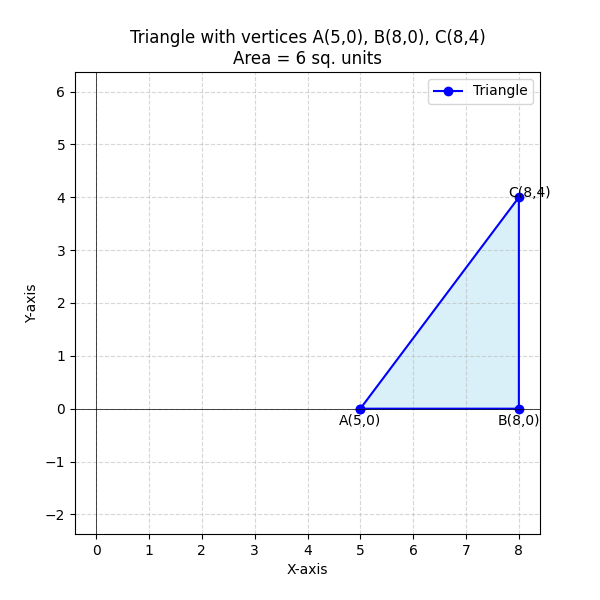
\includegraphics[height=0.6\textheight, keepaspectratio]{figs/q4.png}
\captionof{figure}{Graph of the Triangle}
\end{figure}
\end{frame}

\begin{frame}[fragile]
    \frametitle{C Code}
\begin{lstlisting}
#include <stdio.h>
#include <math.h>  // for fabs

// Function to compute area of a triangle given three vertices
double triangle_area(double x1, double y1,
                     double x2, double y2,
                     double x3, double y3)
{
    double area = fabs(x1 * (y2 - y3) +
                       x2 * (y3 - y1) +
                       x3 * (y1 - y2)) / 2.0;
    return area;
}
int main() {
    // Given vertices
    double x1 = 5, y1 = 0;
    double x2 = 8, y2 = 0;
    double x3 = 8, y3 = 4;

\end{lstlisting}
\end{frame}

\begin{frame}[fragile]
    \frametitle{C Code}
\begin{lstlisting}
    double area = triangle_area(x1, y1, x2, y2, x3, y3);

    printf("The area of the triangle is: %.2f sq.units\n", area);

    return 0;
}
\end{lstlisting}
\end{frame}

\begin{frame}[fragile]
    \frametitle{Python Code}
\begin{lstlisting}
import numpy as np
import matplotlib.pyplot as plt

# Triangle vertices
A = (5, 0)
B = (8, 0)
C = (8, 4)

# Extract x and y coordinates for plotting
x_coords = [A[0], B[0], C[0], A[0]]  # Close the triangle by returning to A
y_coords = [A[1], B[1], C[1], A[1]]

# Plot the triangle
plt.figure(figsize=(6,6))
plt.plot(x_coords, y_coords, 'bo-', label='Triangle')
plt.fill(x_coords, y_coords, 'skyblue', alpha=0.3)  # shaded area

# Label the points

\end{lstlisting}
\end{frame}

\begin{frame}[fragile]
    \frametitle{Python Code}
\begin{lstlisting}
plt.text(A[0], A[1]-0.3, 'A(5,0)', ha='center')
plt.text(B[0], B[1]-0.3, 'B(8,0)', ha='center')
plt.text(C[0]+0.2, C[1], 'C(8,4)', ha='center')

# Add grid, axis, and title
plt.axhline(0, color='black', linewidth=0.5)
plt.axvline(0, color='black', linewidth=0.5)
plt.grid(True, linestyle='--', alpha=0.5)
plt.xlabel('X-axis')
plt.ylabel('Y-axis')
plt.title('Triangle with vertices A(5,0), B(8,0), C(8,4)\nArea = 6 sq. units')
plt.axis('equal')  # Equal scaling on both axes
plt.legend()
plt.savefig("/home/arsh-dhoke/ee1030-2025/ee25btech11010/matgeo/2.7.22/figs/q4.png")
plt.show()
\end{lstlisting}
\end{frame}

\begin{frame}[fragile]
    \frametitle{Python+ C Code}
\begin{lstlisting}
import ctypes
import numpy as np
import matplotlib.pyplot as plt

# ==============================
# Load C shared library
# ==============================
lib = ctypes.CDLL("./code.so")

# Define function signature
lib.triangle_area.argtypes = [ctypes.c_double, ctypes.c_double,
                              ctypes.c_double, ctypes.c_double,
                              ctypes.c_double, ctypes.c_double]
lib.triangle_area.restype = ctypes.c_double

# Triangle vertices
A = (5.0, 0.0)
B = (8.0, 0.0)
C = (8.0, 4.0)

\end{lstlisting}
\end{frame}

\begin{frame}[fragile]
    \frametitle{Python+ C Code}
\begin{lstlisting}
# Compute area using the C function
area = lib.triangle_area(A[0], A[1], B[0], B[1], C[0], C[1])
print(f"Area of the triangle (from C): {area:.2f} sq.units")

# ==============================
# Plotting the triangle
# ==============================
x_coords = [A[0], B[0], C[0], A[0]]  # close the triangle
y_coords = [A[1], B[1], C[1], A[1]]

plt.figure(figsize=(6,6))
plt.plot(x_coords, y_coords, 'bo-', label='Triangle')
plt.fill(x_coords, y_coords, 'skyblue', alpha=0.3)

# Label the points
plt.text(A[0], A[1]-0.3, f'A{A}', ha='center')
plt.text(B[0], B[1]-0.3, f'B{B}', ha='center')
plt.text(C[0]+0.2, C[1], f'C{C}', ha='center')
\end{lstlisting}
\end{frame}

\begin{frame}[fragile]
    \frametitle{Python+ C Code}
\begin{lstlisting}
# Add grid, axis, and title
plt.axhline(0, color='black', linewidth=0.5)
plt.axvline(0, color='black', linewidth=0.5)
plt.grid(True, linestyle='--', alpha=0.5)
plt.xlabel('X-axis')
plt.ylabel('Y-axis')
plt.title(f'Triangle with vertices A{A}, B{B}, C{C}\nArea = {area:.2f} sq. units')
plt.axis('equal')
plt.legend()
plt.savefig("/home/arsh-dhoke/ee1030-2025/ee25btech11010/matgeo/2.7.22/figs/q4.png")
plt.show()
\end{lstlisting}
\end{frame}
\end{document}